\section{Firewall}
The firewall is an important factor in security. Open or incorrectly configured ports can quickly make a server vulnerable, especially if you have other components running on it.
The firewall was tested with nmap \cite{nmap-portscan}


\subsubsection{BEFORE script}
It should also be mentioned that the ``before'' run looks worse than the ``after'' run at first sight (more open ports). 
This is because ports needed for the components must be opened. The rest of the traffic is safely closed for this, so the server owner has control over it.

\begin{figure}[H]
	\centering
	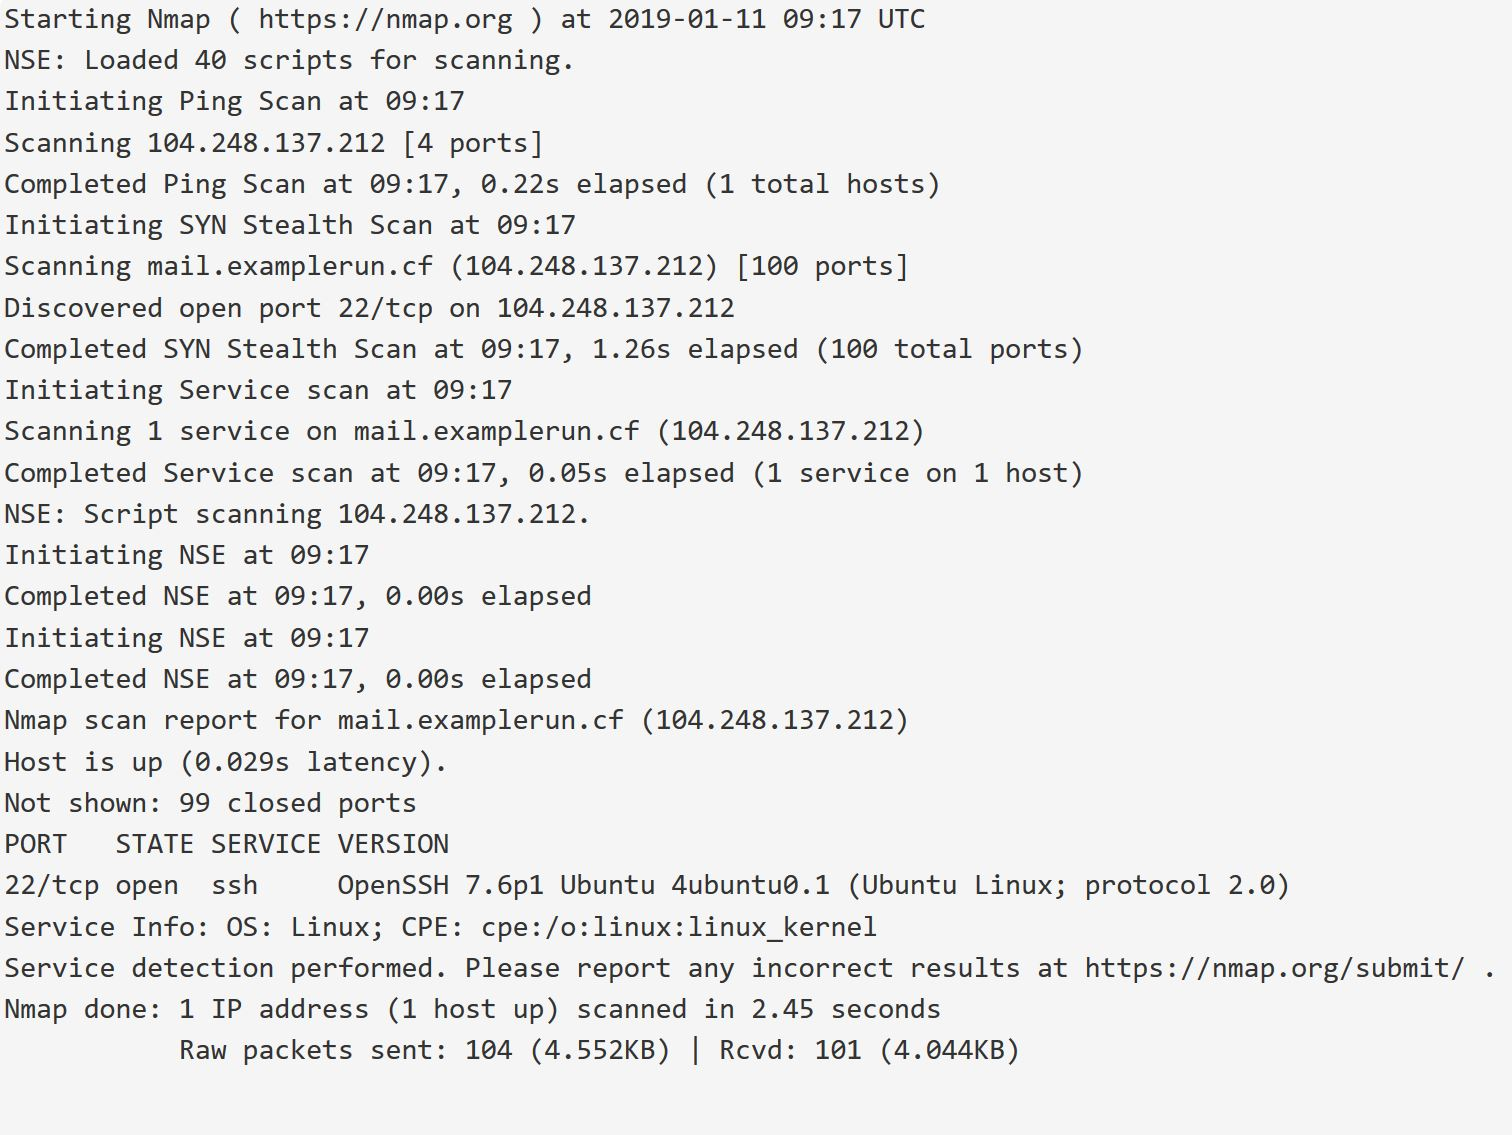
\includegraphics[width=\linewidth]{pics/fw_before_no_dns}
    \caption{Firewall (without DNS) \textbf{BEFORE}}
	\label{fig:firewallnodnsbefore}
\end{figure}

\begin{figure}[H]
	\centering
	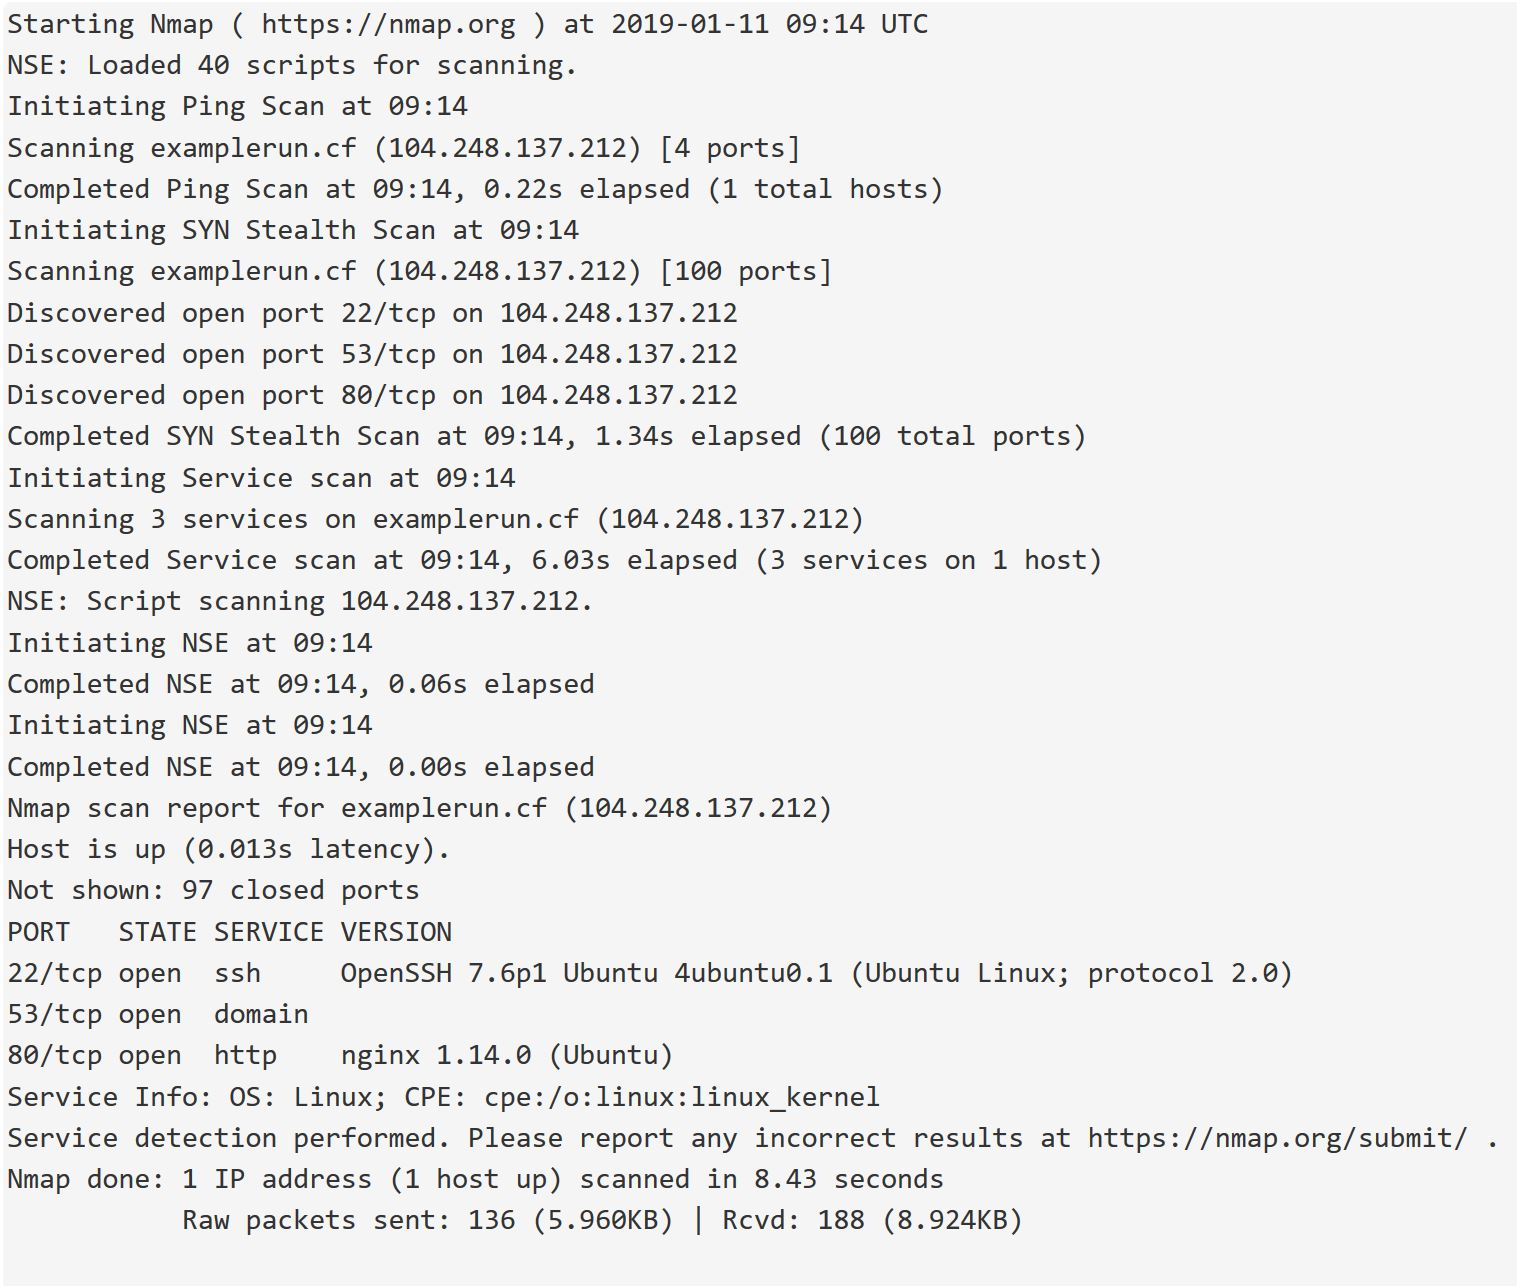
\includegraphics[width=\linewidth]{pics/fw_before_with_dns}
    \caption{Firewall (with DNS) \textbf{BEFORE}}
	\label{fig:firewallwithdnsbefore}
\end{figure}


\subsubsection{AFTER script}

\begin{figure}[H]
	\centering
	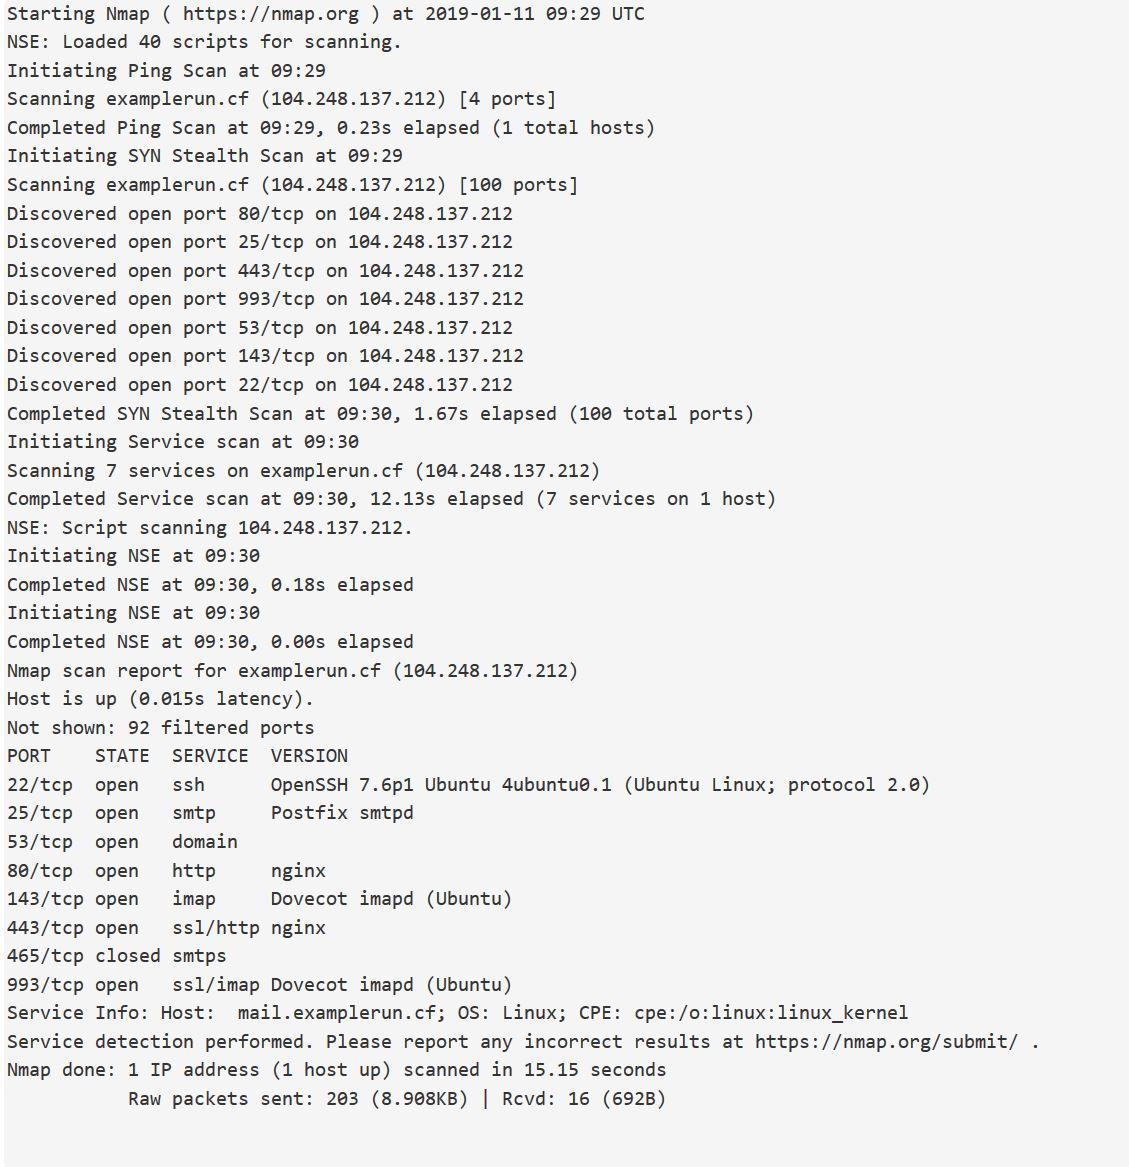
\includegraphics[width=\linewidth]{pics/fw_after}
	\caption{Firewall setup \textbf{AFTER}}
	\label{fig:firewallafter}
\end{figure}
\newpage
